\documentclass[10pt,twocolumn,letterpaper]{article}

\usepackage{cvpr}
\usepackage{times}
\usepackage{epsfig}
\usepackage{graphicx}
\usepackage{amsmath}
\usepackage{amssymb}
\usepackage{eurosym}
\usepackage{amsmath}

\DeclareMathOperator*{\argmax}{\arg\!\max}
\DeclareMathOperator*{\argmin}{\arg\!\min}

% 1st arg: Author. 2nd arg: Label
\newcommand{\cit}[2]{#1 \textit{et al.} \cite{#2}}

\newcommand*{\thead}[1]{\bfseries #1} 

% Include other packages here, before hyperref.

% If you comment hyperref and then uncomment it, you should delete
% egpaper.aux before re-running latex.  (Or just hit 'q' on the first latex
% run, let it finish, and you should be clear).
\usepackage[citecolor=black,pagebackref=true,breaklinks=true,letterpaper=true,colorlinks=true,linkcolor=black,bookmarks=false]{hyperref}

\cvprfinalcopy % *** Uncomment this line for the final submission

\def\cvprPaperID{****} % *** Enter the CVPR Paper ID here
\def\httilde{\mbox{\tt\raisebox{-.5ex}{\symbol{126}}}}

% Pages are numbered in submission mode, and unnumbered in camera-ready
\ifcvprfinal\pagestyle{empty}\fi
\begin{document}

%%%%%%%%% TITLE
\title{Face2Face: an innovative way to face recognition \\ DL-IC 2018 Project} 

\author{D'Amico Edoardo\\
Politecnico di Milano\\
{\tt\small edoardo.damico@polimi.it}
% For a paper whose authors are all at the same institution,
% omit the following lines up until the closing ``}''.
% Additional authors and addresses can be added with ``\and'',
% just like the second author.
% To save space, use either the email address or home page, not both
\and
Gabbolini Giovanni\\
Politecnico di Milano\\
{\tt\small giovanni.gabbolini@polimi.it}
\and
Parroni Federico\\
Politecnico di Milano\\
{\tt\small federico.parroni@polimi.it}
}

\maketitle
%\thispagestyle{empty}

%%%%%%%%% ABSTRACT
\begin{abstract}
In this paper we present a method to compare two images and get a similarity measure of these. Common usages of such a technique are several, first of all, authentication and face matching.
\\
This system, called Face2Face, uses a deep convolutional neural network to map a couple of images into a vector of features which capture the similarity between the two images. Then, this vector is processed by the last fully-connected layers of the network which output a measure in the range [0,1] representing the probability of having depicted the same person on the two images. Training has been done by stacking couples of images one on top of the other, exploiting convolution filters in order to capture face similarities. This method boosts also the size of the training set: in fact, each image of the N in the training set can be coupled with all the others, so the training samples that can be obtained $\in O(N^2)$.
\\
The main benefit of this mechanism are essentially the almost absence of hardware needed (only a camera) and the ease of use for the actual implementation. 
\end{abstract}

%%%%%%%%% BODY TEXT
%------------------------------------------------------------------------

\section{Introduction}

Nowadays, authentication is one of the most critical point of computer security. Authentication is a mechanism that allows a user to exhibit a proof of his identity in order to be recognized by a particular system. Aim of this project is to implement a biometric authentication software, based on face recognition, using a convolutional neural network. The only hardware requirement is a camera. The process of authentication is composed by the following steps:
\begin{itemize}
\item User records a set of photos of himself (sample photos) and saves them into the system
\item When user wants to authenticate, the system asks for a photo
\item If the similarity between the sample photos and the current one is greater than a fixed threshold, user is authenticated positively
\end{itemize}
The main advantage of this approach is the cost/performance tradeoff that we can achieve: currently, costs of commercial biometric scanners are in the order of hundreds of euros, while a suitable camera for this technique costs about 10-20\euro \, and the probability of granting access to a wrong user is in the order of 1 over 1000.

This work should provide a different approach from the current state of the art to compare two images using a deep convolutional neural network, resulting in a lightweight and real-time process. The neural network takes as input two images and outputs a similarity value between 0 and 1, so it can be directly used without other intermediate softwares. The methodolody used to train the network requires a quite low number of photos to build a large amount of training samples, as described later in \ref{sec:exp}.


\section{Related work}
%In this section you should discuss published work that relates to your project. This is expected to be full of references, meaning that you have read the existing literature and you know what you are working on very well. This is not just a list or works, but you are not supposed to cluster papers that use similar approaches and compare them each other using very short sentences. I strongly suggest to check \cite{steinhardt, lipton} blog posts for some good practices in writing a paper. A quote that I like very much is \emph{``Research is spending 6 hours reading 35 papers, so you can write one sentence containing 2 references''} \cite{twit:ref}. Keep it in mind while you are writing!
%------------------------------------------------------------------------
Our work is based on training a deep convolutional neural network, using a purely data driven approach, to extract features from couple of images than use it as input to a fully connected network to say wheter two images representing faces are of the same person or not.
Similar work has been carried out some using directly deep convolutional neural network to give a response other using it as a support for the extraction of features used as input for SVMs.
\\
The most relevant are reported below.
\\
\par
Schroff \textit{et al.} [] use a deep convolutional neural network to generate an embedding $f(x)$, from an image $x$ into a feature space $R^d$, such that the squared distance between all faces of the same identity is small, whereas the squared distance between a pair of face images from different identities is large. To achieve that has been used the so called 'triplet loss' that allows the faces for one identity to live on a manifold, while still enforcing the distance of two different faces to be maximum.
The work presented does not directly solve the problem of the face recognition but create a proper enviroment in which a simple K-NN classifier can solve the task.
\\
\par
Aleju \cite{aleju} The network presented uses two branches, one per image. Each branch applies a few convolutions and ends in a fully connected layer. The outputs of both branches are then merged and further processed by another fully connected layer, before making the final yes-no-decision (whether both images show the same person).
\\
\par
\cit{Taigman}{taigman} propose a multi-stage approach that aligns faces to a general 3D shape model. A multi-class net-work is trained to perform the face recognition task on over four thousand identities. The authors also experimented with a so called Siamese network where they directly opti-
mize the $L1$-distance between two face features. Their best performance on LFW (97.35\%) obtained from an ensemble of three networks using different alignments and color channels. The predicted distances (non-linear SVM predictions) of those networks are combined using a non-linear SVM.
\\
\par
\cit{Zhenyao}{zhenyao} employ a deep network  to “warp” faces into a canonical frontal view and then learn CNN that classifies each face as belonging to a known identity. For face verification, PCA on the network output in conjunction with an ensemble of SVMs is used.


\section{Proposed approach}
To accomplish our work we used a convolutional neural network. This kind of model is nowadays the most widely used for Image Recognition tasks. Many ways have been proposed to tackle the problem of stating similarity among different images, for example \cit{Schroff}{google}. Our solution is based on the idea of using directly convolutional layers to extract similarity, which is in our case expressed in terms of identity of people. In order to follow this idea, we used as input of our convolutional neural network two gray scale images stacked one upon the other. Then, two-dimensional convolutional layers filter those two levels images, transforming the initial input. The vector which comes from the flattenization of the last convolutional layer output represents an embedding of the initial input which would naturally tell the relation between the two images in terms of similarity among identities of people appearing in those. Then the vector of features is used as input of a fully connected neural network, which will, at the really end, output a number between 0 and 1, \ie the probability of having two photos who depict the same person.

\begin{figure}[t]
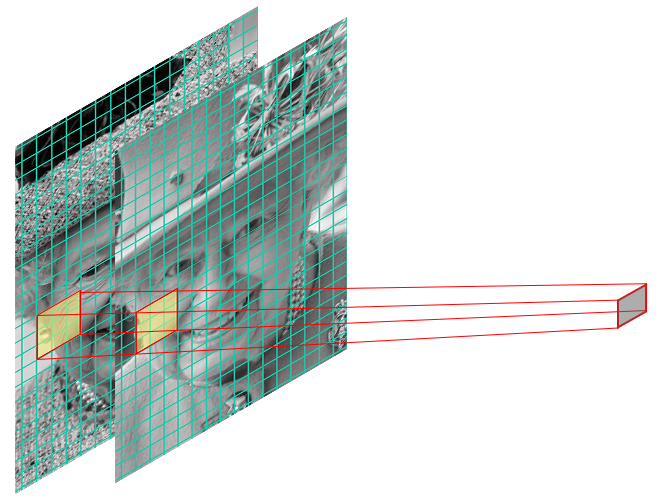
\includegraphics[width=0.8\linewidth]{images/stackedconvolution.png}
   \caption{Convolution between two stacked image. Large convolution filters can help to capture similiarities.}
\label{fig:long}
\label{fig:onecol}
\end{figure}

%-------------------------------------------------------------------------
\subsection{Mathematics}
We can consider training samples as i.i.d observations from a Bernoulli random variable. We want that our model approximates as well as possible this Bernoulli variable ($t_n$ can assume only values $0$ or $1$):
\begin{equation}
P(t_n = 1|x_n, \textbf{w}) = y(x_n)
\end{equation}
where $y(x_n)$ is the output of the convolutional neural network for the $n^{th}$ sample.
\\
We want to maximize the likelihood of getting the right ouput. To do so, we have to choose the vector of coefficients $\textbf{w}$ such that:
\begin{equation}
\argmax _{\textbf{w}} J(\textbf{w}) = \argmax _{\textbf{w}} \prod _n^N {y_n}^{t_n}(1-y_n)^{1-t_n}
\end{equation}
Passing to the negative log, we get the standard binary crossentropy:
\begin{equation}
\argmin _{\textbf{w}} J(\textbf{w}) = - \sum _{n=1}^{N}\ {\bigg [}t_{n}\log {y_n}+(1-t_{n})\log(1-{y_n}){\bigg ]}
\end{equation}

%-------------------------------------------------------------------------

\subsection{Model Selection}
The model selection has been one of the main challanges during our activity: we did not have other already existing works from which transfer the structure of the network, at least no other research product which was using the same approach to achieve the same goal. So first we decided to go for a Cross Validation among the possible models. Even if the amount of data that we managed to harvest (\ref{subsubsec:ownd}) was enough to proceed with this idea, the methodology appeared to be computationally unfeasible. So we decided to go for a standerd validation approach. Of course we did not validate every possible model but instead we listed a set of fifteen networks of growing complexity. As a guideline for this ranking we have mainly considered \cit{Bengio}{hypsel}
To have the most unbiased estimate of the true error from our validation set, we randomly split the data into validation and training set before the actual validation procedure, and before any of the candidate network was trained and evaluated on the data.
When validating the various models, we used Adam Optimizer: this guaranteed to be free from the choice of the learning rate, removing one degree of freedom from our validation procedure.
The resulting model is presented in Table 1.
\\
\begin{table}[]
\label{tab:model}
\begin{center}
\begin{tabular}{l|l|l|l}
\thead{Layer} & \thead{Kernel} & \thead{Output shape} & \thead{\# of params} \\
\hline
Conv2D  & 3x3 (16) & (80, 80, 16)  & 304               \\
\hline
MaxPooling2D & 2x2 & (40, 40, 16)  & 0                \\
\hline
Dropout   & p=0.1 & (40, 40, 16)  & 0                \\

\hline
Conv2D    & 3x3 (16) & (40, 40, 16)  & 2320              \\
\hline
MaxPooling2D & 2x2 &(20, 20, 16)  & 0                \\
\hline
Dropout   & p=0.1 & (20, 20, 4)  & 0                \\

\hline
Conv2D   & 3x3 (16) & (20, 20, 16)  & 2320              \\
\hline
MaxPooling2D & 2x2 & (10, 10, 16)  & 0                \\
\hline
Dropout   & p=0.1 & (10, 10, 16)  & 0                \\

\hline
Conv2D    & 3x3 (16) & (10, 10, 16)  & 2320              \\

\hline
Flatten      & (1600)         & 0                \\

\hline
Dense   & 128 & (128)           & 204928          \\
\hline
Dropout  & p=0.1 & (128)           & 0                \\
\hline
Dense   & 128 & (128)           & 16512             \\
\hline
Dense   & 128 & (128)           & 16512                \\
\hline
Dense (softmax) & 2 & (2)            & 258              \\
\hline
\multicolumn{3}{l}{Total}   & 245474         
\end{tabular}
\end{center}
\caption{Structure of the network}
\end{table}
\\
All the models have been trained for threehundred epochs changing dinamically the training data: when the model started overfitting \ie when the training and test error were starting to be uncorrelated, we swapped to a different training set, sampled from the whole set of training samples. Every sampled chunk counted roughly fifty thousand couples of images. This technique was on one hand necessary, because the whole dataset was not fitting on memory, and on the other hand turned out to be a powerful regularization tool.

%
%When placing figures in \LaTeX, it's almost always best to use
%\verb+\includegraphics+, and to specify the  figure width as a multiple of
%the line width as in the example below
%{\small\begin{verbatim}
%   \usepackage[dvips]{graphicx} ...
%   \includegraphics[width=0.8\linewidth]
%                   {myfile.eps}
%\end{verbatim}
%}

%------------------------------------------------------------------------


\section{Experiments}
%In this section you validate your method showing the experiments that you performed. The experiments will vary depending on the project, but you might compare with previously published methods, perform an ablation study to determine the impact of various components of your system, experiment with different hyperparameters or architectural choices, use visualization techniques to gain insight into how your model works, discuss common failure modes of your model, etc. You should include graphs, tables, or other figures to illustrate your experimental results. Divide in subsections or paragraphs to help the reader navigate in your paper.

\subsection{Evaluation}
We have evaluated our method on a test set that accounts for approximately the 20\% of the intial dataset that we gathered up, so the test data has the same distribution of our training set, but disjoint identities.
The model has been evaluated also on two different test sets, the YLF and YTBF for comparing it to the state of the art level of face recognition. 
\paragraph{}
A substantial between the training and test set images is that the test set has not been augmented so that the evaluation of the performance can unbiased with respect to the training set as much as possible, augmentation has been performed only on the training set (see next subsection).
\paragraph{}
we have evaluated the method on the face verification task (say wheter two face images are representing the same person) using as prediction the output of the net $Y(i,j)$ representing the $probability$ of having the same person on the two images. All faces pairs $(i,j)$ of the same identity are denoted with $N_{same}$, whereas all pairs of different identities are denoted with $N_{diff}$.\\
 
We define the set of all \textit{true accepts} as
\begin{equation}
TA(thld)=\{(i,j) \in N_{same}, with Y(i,j) > thld\}
\end{equation}
these are the face pairs $(i,j)$ that were correctly classified at treshold $thld$.
Similarly we can define the \textit{False accepts} as 
\begin{equation}
FA(thld)=\{(i,j) \in N_{diff}, with Y(i,j) > thld\} 
\end{equation}
is the set of all pairs that was missclassified as \textit{same}, this figure of merit has a main role on the evaluation of our work since the method as been created with the aim of being used as a security check so the false accepts can not be tolerated.
\paragraph{Obtained performance}
after 5/6 hours of training (200 epochs) we have reached a
\begin{equation}
validationaccuracy = 0.81 with thld = 0.5
\end{equation}
For evaluate the generalization performance the ROC curve and the AUC parameter has been considered.

\begin{figure}[t]
\begin{center}
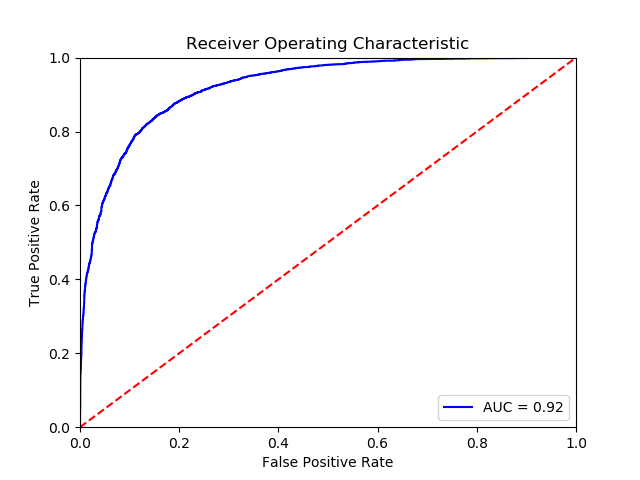
\includegraphics[width=0.8\linewidth]{images/ROC.png}
   \caption{ROC curve of the model.}
\label{fig:long}
\label{fig:onecol}
\end{center}
\end{figure}

the $AUC$ obtained is 0.92 and from the ROC curve we can extract important information on which value the treshold of the model has to be set depending on the utilization purpose of the net.
Since the model has been developed for security reasons a possible idea is to tolerate at most a 10\% of false positive to achieve that the treshold has to be set to 0.9 as suggested by the ROC curve, so that the network will recognize a couple of faces $(i,j)$ as the same person only when $Y(i,j)>0.9$. The performance between two different tresholds can be compared using the confusion matrices taking into account also the
\begin{equation}
Precision(thld) = \frac{TA(thld)}{TA(thld)+FA(thld)}. 
\end{equation}
 
 
%\begin{figure}[t]
%\begin{center}
%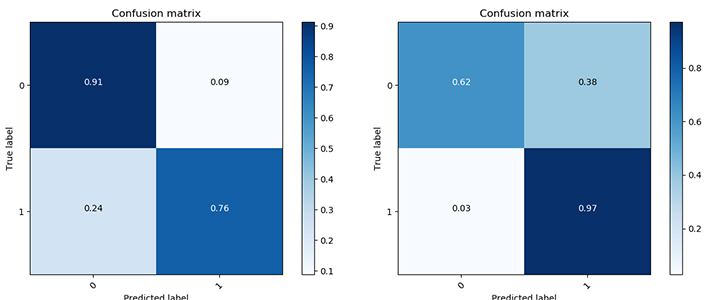
\includegraphics[width=0.8\linewidth]{images/conf_matrix.jpg}
%   \caption{comparison between the confusion matrix with two different tresholds 0.5(on the left) and 0.9}
%\label{fig:long}
%\label{fig:onecol}
%\end{center}
%\end{figure}

\begin{figure*}
\begin{center}
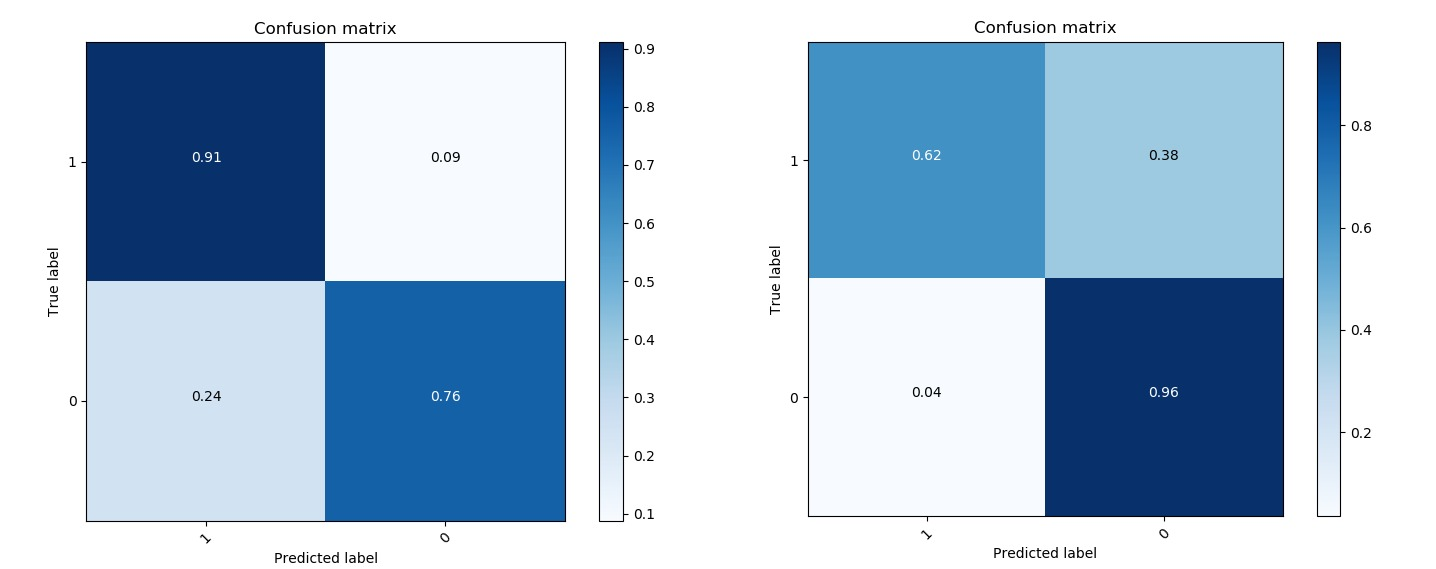
\includegraphics[width=1\linewidth]{images/cm.jpg}
\end{center}
   \caption{comparison between the confusion matrix with two different tresholds 0.5(on the left) and 0.9}
\label{fig:conf_matrices}
\end{figure*}


\begin{table}[]
\centering
\begin{tabular}{|c|ll|}
\hline
Treshold & Accuracy & Precision \\ \hline
0.5                          & 0.835    & 0.791     \\ \hline
0.9                          & 0.795    & 0.953     \\ \hline
\end{tabular}
\end{table}


The accuracies obtained changing the two tresholds are comparable but the $precision$ is considerably higher(20\%) when the treshold is set to 0.9.

\subsection{Datasets}
\subsubsection{Own Dataset}
We gathered our own data through a web page \cite{gdpdataret} that we set up. Through it, people had the possibility to upload their own photos. As a result, we obtained a set of more than eighty folders of photos, each one belonging to a different person. On avarage, we managed to get ten photos per person. Those photos are characterized by really regular poses of the person depicted in it, because the contributors were explicitly asked in the website to shot the photos keeping the camera in from of them, while they were watching it.
\paragraph{Data Augmentation}
The quantity of data that we obtained is not even close to the usual amount used in large scale Deep Learning projects. So we proceeded with augmentation procedures of our training set. In particular we resorted to the Augumentor Python library \cite{augmentor}. This library allows to generate, starting from a set of images, other images, obtained from various transformations of the former set. Those transformations can be customized and can be applied randomly to each image. It follows that each augmented image is the combination of the application of a random number of transformation specified by the developer, resulting in a great variety in the augmented set.
The transformation applied, with probabilities, are:
\begin{itemize}
\item Flip left-right with probability 0.5;
\item Skew left-right with probability 1: the skew magnitude is random and varies from 0 to 0.2, which experimentally guarantees resulting images which are not deformed;
\item Alter brightness with probability 1: we perform a non linear trasformation as suggested in \cite{nonlintransf}, using parameters $\theta = 1$ and $\phi = 1$ respectively. In particular we used this transformation increasing the pixel brightness and decreasing it with probability 0.5 in both cases;
\item Adaptive equalization \cite{histeq} with probability 0.5, using a clip limit of 0.01;
\end{itemize}
In particular the last two methods were employed in order to obtain more variety of lightning conditions, which turned out to be characteristic that was lacking the most in our own dataset.
Using this augmentation procedure, we crafted five brand new images from just one, obtaining fifty images per person on our dataset.

\begin{figure}[t]
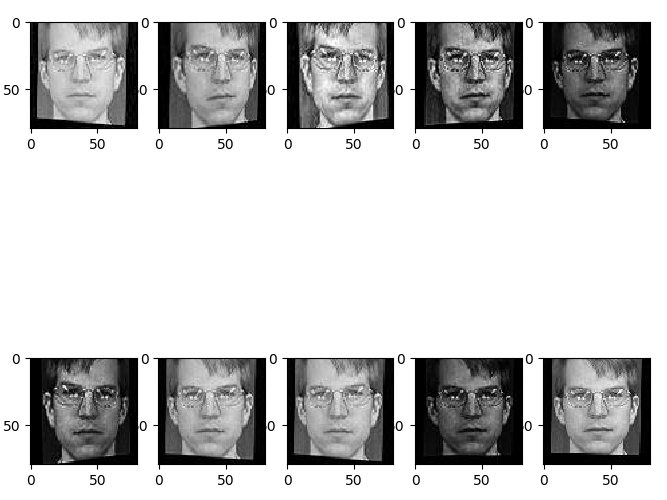
\includegraphics[width=1\linewidth]{images/augmented.png}
   \caption{Example of nine augmented photos obtained from a starting one, which is depicted at the bottom-right. We can see the good variety of images obtained from our augmentation procedure.}
\label{fig:long}
\label{fig:onecol}
\end{figure}

\paragraph{Data preprocessing}
The data that we managed to harvest and the results of the augmentation procedure were affected by noise and really low regularity. To hope to get good results, we needed to have all the images in a standardized form factor. To accomplish this idea, we set up a pipeline useful to apply to all the images those following steps:

\begin{enumerate}
\item Find the face in the image and crop everything else
\item Resize the image to a standard size
\item Rotate the image in order to get the person eye in a standard position
\end{enumerate}

Finding a face in an image and pick the bounding box which includes it is a really known task in Computer Vision and really efficient and reliable algorithms exist. We resorted to the HOG Algorithm \cite{hog}. A more tough problem is rotating an image so that the eyes are aligned at the same position, however a detailed description of how to tackle this problem can be found in \cite{facealign}

\begin{figure}[t]
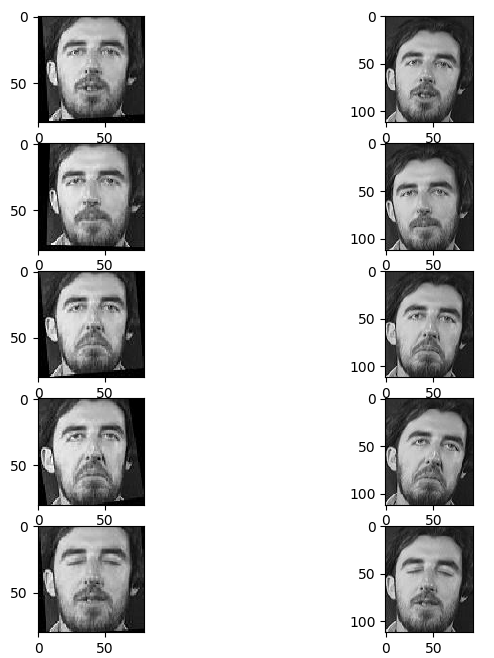
\includegraphics[width=1\linewidth]{images/processed.png}
   \caption{Examples of the application of the pipeline. On the left we see the processed images, on the right we have the original ones. We see the difference of sizing, the eye alignment and the face that has been cropped}
\label{fig:long}
\label{fig:onecol}
\end{figure}

\paragraph{Couple creation}
At this point, we have a considerable number of folders, one for each identity, each one containing a set of, on avarage, fifty augmented photos. Still, we are missing our actual dataset, which is composed of couples of images and a labels: if the two photos come from the same folder, then the label will be Zero, otherwise One. Since we are considering couples, the number of training samples grows not linearly with the number of photos, but quadratically: for any photo in a folder, we can pair it with all the other photos on the folder and with an equal number of photos picked from other random folders. In formulas, a folder with $N$ photos will give $2(N-1)^2$ training samples.
Using this trick, at the really end we managed to have a dataset with more than one million samples.

%Describe the data you are working with for your project. Usually you need to explain what type of data is it, how much data are you working with and if you applied any pre-processing, filtering, or other special treatment to use it. Remember that you have to cite each dataset you used in your project if it has been published from someone else. Instead, if you collected it by yourself you have to describe accurately how you gathered (and labeled) your data.

\subsubsection{Academic Datasets}
\paragraph{Labelled Faces in the Wild} We have validated the performance of our network in this well known dataset. We have built the couples and assigned the labels as we did in our own dataset, and then evaluated the accuracy.

\subsubsection{Performance}

\begin{figure}[t]
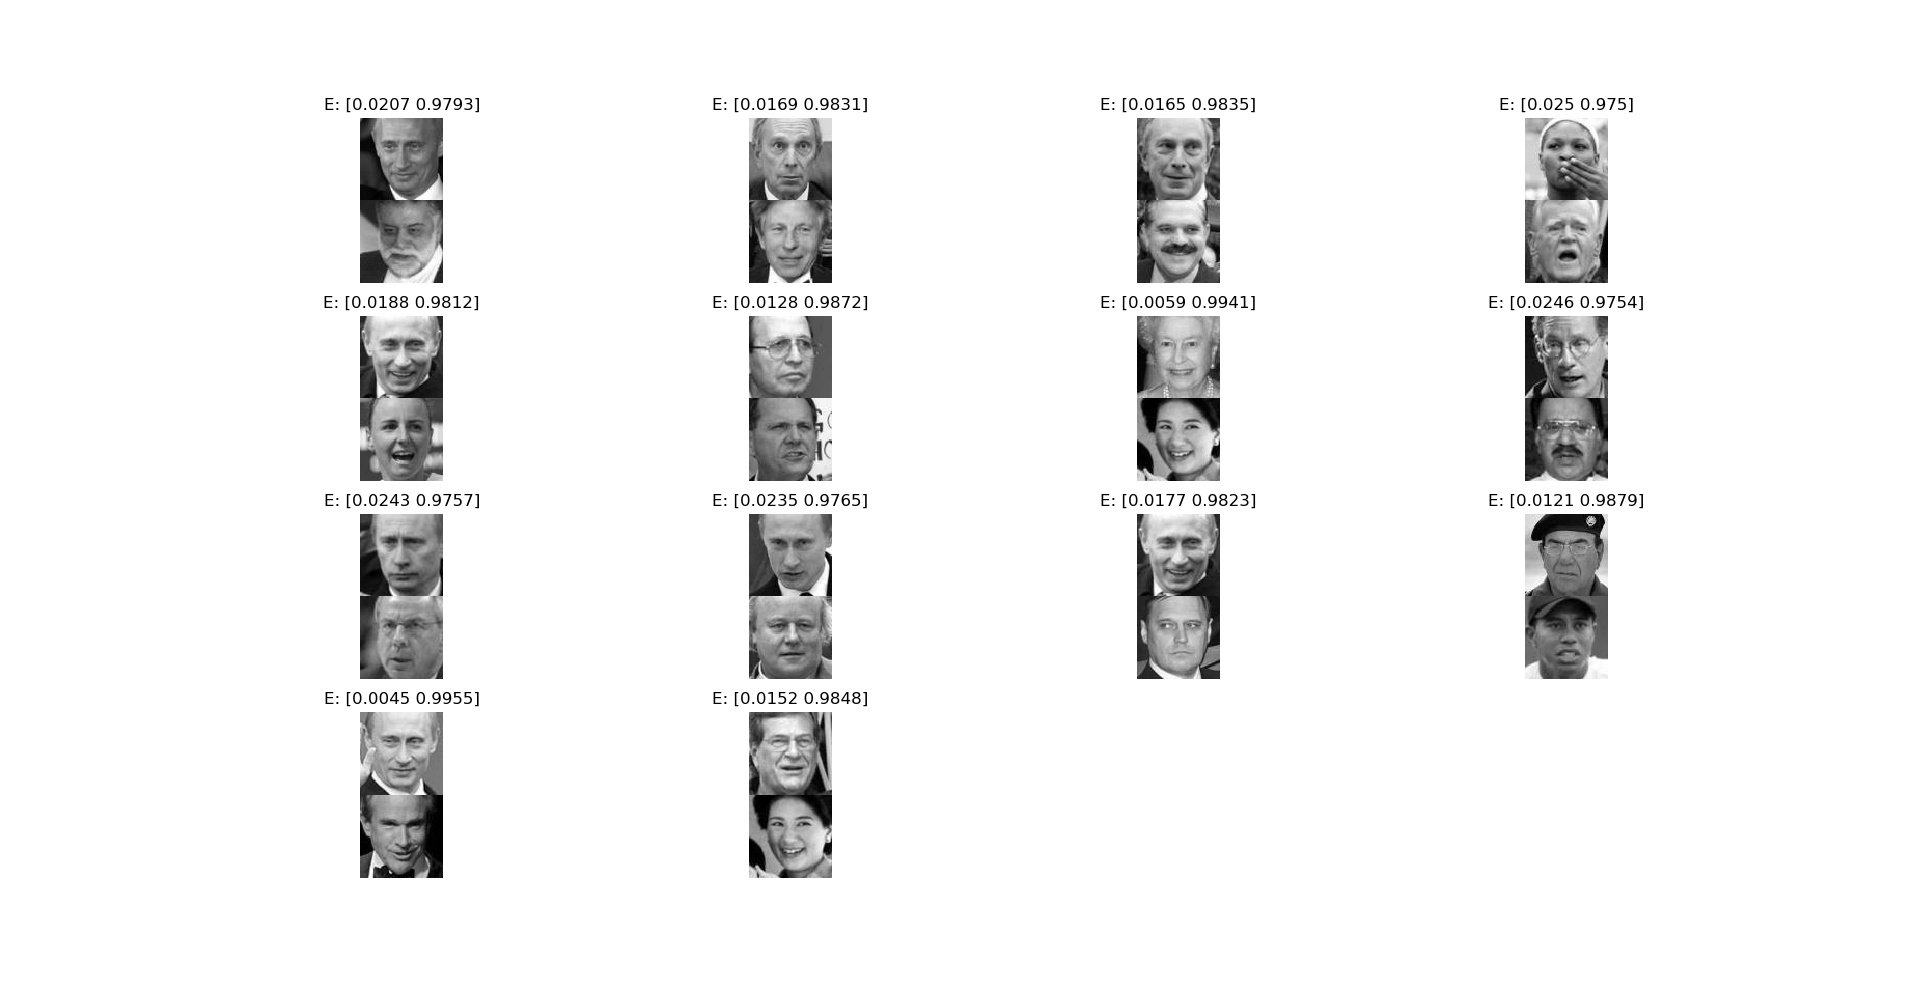
\includegraphics[width=1\linewidth]{images/falsepositive.jpg}
   \caption{Examples of false positive training samples, obtained with a threshold equals to $0.9$. On top of each couple we have the prediction of the network \ie the second number, but all those images were labelled as 0, infact they depict the same person}
\label{fig:long}
\label{fig:onecol}
\end{figure}

\paragraph{Experiments setup.}
Here you describe all the architectural choices of your model, the hyper-parameters of your model, \eg optimizer, learning rate, momentum, batch size and if you cross-validate on them. 

\paragraph{Results and discussion.}
Discuss your results and compare with other methods. You can also perform an \emph{ablation study} on your model switching on and off some components to understand their contributions.


\section{Conclusion} 
Summarize your key results. What have you learned from the project and suggest future extensions or new applications of your ideas.


\begin{figure}[t]
\begin{center}
\fbox{\rule{0pt}{2in} \rule{0.9\linewidth}{0pt}}
   %\includegraphics[width=0.8\linewidth]{egfigure.eps}
\end{center}
   \caption{Example of caption.  It is set in Roman so that mathematics
   (always set in Roman: $B \sin A = A \sin B$) may be included without an
   ugly clash.}
\label{fig:long}
\label{fig:onecol}
\end{figure}


\begin{figure*}
\begin{center}
\fbox{\rule{0pt}{2in} \rule{.9\linewidth}{0pt}}
\end{center}
   \caption{Example of a short caption, which should be centered.}
\label{fig:short}
\end{figure*}

%-------------------------------------------------------------------------


\section*{Acknowledgements}
We would like to thank all the people that contributed with their own photos to our project, which made our work concretely possible.

%-------------------------------------------------------------------------
\begin{thebibliography}{9}

\bibitem{google} 
Florian Schroff, Dmitry Kalenichenko and James Philbin
\textit{FaceNet: A unified embedding for face recognition and clustering}.

\bibitem{hypsel}
Yoshua Bengio
\textit{Practical Recommendations for Gradient-Based Training of Deep
Architectures}

\bibitem{gdpdataret}
\textit{http://keyblade95.altervista.org/faceupload/}

\bibitem{augmentor}
\textit{https://github.com/mdbloice/Augmentor}

\bibitem{nonlintransf}
\textit{https://stackoverflow.com/questions/19363293/whats-the-fastest-way-to-increase-color-image-contrast-with-opencv-in-python-c}

\bibitem{histeq}
\textit{https://towardsdatascience.com/image-augmentation-for-deep-learning-using-keras-and-histogram-equalization-9329f6ae5085}

\bibitem{hog}
\textit{https://www.learnopencv.com/histogram-of-oriented-gradients/}

\bibitem{facealign}
\textit{https://www.pyimagesearch.com/2017/05/22/face-alignment-with-opencv-and-python/}

\bibitem{aleju}
\textit{https://github.com/aleju/face-comparer}

\bibitem{taigman}
\textit{Y. Taigman, M. Yang, M. Ranzato, and L. Wolf. Deepface:
Closing the gap to human-level performance in face verification.}

\bibitem{zhenyao}
\textit{Z. Zhu, P. Luo, X. Wang, and X. Tang. Recover canonical view
faces in the wild with deep neural networks.}

\bibitem{repo}
\textit{https://github.com/keyblade95/DeepLearningProject/}

\end{thebibliography}

\end{document}
